% CVSId: $Id: oqe.tex,v 1.3 2002-04-29 23:07:50 cananian Exp $
\documentclass[%
pdf,
colorBG,
slideColor,
%nocolorBG,
%slideBW,
%%%%%%%%%%%%%%%%%%%%%
nototal,
%distiller,
%%%%%%%%%%%%%%%%%%%%%
%draft,
oqe
%frames
%azure
%contemporain
%nuancegris
%troispoints
%lignesbleues
%darkblue
%alienglow
%autumn
]{prosper}
\usepackage{amsmath}
\usepackage{comdef}\newcommand{\figscale}{1.0}
\usepackage{pst-node}
\hypersetup{pdfpagemode=FullScreen}

\title{Size Optimizations for Java Programs}
%\author{\href{http://cscott.net}{C.~Scott~Ananian}}
\author{C.~Scott~Ananian}
\email{cananian@lcs.mit.edu}
\institution{%
Laboratory for Computer Science\\
Massachusetts Institute of Technology}

%\DefaultTransition{Wipe}

\begin{document}
\maketitle

%---------------------------------------------------------------------- SLIDE -
% \begin{slide}{The quest for $\pi$}
% \begin{itemize}
% \item The following formula computes $8$ correct digits per iteration 
%   (Ramanujan):
% \end{itemize}
%   \begin{small}
%   \begin{equation*}
%     \frac{1}{\pi}=\sum_{n=0}^\infty \frac{(\frac{1}{4})_n(\frac{2}{4})_n(\frac{3}{4})_n}{n!^3}\bigl(2\sqrt{2}(1103+26390n)\bigr)\frac{1}{(99^2)^{2n+1}}
%   \end{equation*}
%   \end{small}
% \end{slide}

%---------------------------------------------------------------------- SLIDE -
\begin{slide}{Our Goal}
\begin{center}
Reduce the memory consumption of object-oriented programs

\vspace{0.5cm}
\fontTitle{By}
\vspace{0.5cm}

Using program analysis to identify opportunities to reduce the space
required to store objects,

\vspace{0.5cm}
\fontTitle{Then}
\vspace{0.5cm}

Applying transformations to reduce the memory consumption of the program.
\end{center}
\end{slide}

%---------------------------------------------------------------------- SLIDE -
\begin{slide}{Structure of a Java Object}
\begin{itemize}
\item Typical of many O-O languages.
\end{itemize}
\begin{center}
\includegraphics[scale=0.5]{oqedraw/structure-bbox.eps}
\end{center}
\end{slide}

%---------------------------------------------------------------------- SLIDE -
\begin{slide}{Strategy}
\begin{center}
Push hard on all the bits.

\vspace{0.5cm}
\includegraphics[scale=0.5]{oqedraw/strategy-bbox.eps}
\end{center}
\end{slide}

%---------------------------------------------------------------------- SLIDE -
\newrgbcolor{fieldcomp}{0 1 0}
\newrgbcolor{fieldelim}{0 1 1}
\newrgbcolor{headeropt}{1 0 0}

\overlays{3}{
\begin{slide}{How to compress objects}

Three broad techniques:
%
\parbox[b]{2.5in}{%
\begin{itemize}%
\fieldcomp\renewcommand{\green}{\fieldcomp}% new bullet color
\item Field compression
\fromSlide{2}{
\fieldelim\renewcommand{\green}{\fieldelim}% new bullet color
\item Mostly-constant field elimination
\fromSlide{3}{
\headeropt\renewcommand{\green}{\headeropt}% new bullet color
\item Header optimizations
}}
\renewcommand{\green}{\yellow} % restore yellow bullet color
\end{itemize}
}%
\parbox[b]{1.75in}{%
\onlySlide*{1}{\hspace*{0.106in}\hspace*{0.261in}\includegraphics[scale=0.4]{oqedraw/how-fieldcomp-bbox.eps}}%
\onlySlide*{2}{\hspace*{0.106in}\includegraphics[scale=0.4]{oqedraw/how-fieldelim-bbox.eps}}%
\onlySlide*{3}{\includegraphics[scale=0.4]{oqedraw/how-header-bbox.eps}}%
}%

\end{slide}
}

%---------------------------------------------------------------------- SLIDE -
\begin{slide}{How to compress objects} % just the first one

Three broad techniques:

\parbox[b]{2.5in}{%
\begin{itemize}%
\fieldcomp\renewcommand{\green}{\fieldcomp}% new bullet color
\item Field compression
\lightgray\renewcommand{\green}{\lightgray}% new bullet color
\item Mostly-constant field elimination
\lightgray\renewcommand{\green}{\lightgray}% new bullet color
\item Header optimizations
\renewcommand{\green}{\yellow} % restore yellow bullet color
\end{itemize}
}%
\parbox[b]{1.75in}{%
\hspace*{0.106in}\hspace*{0.261in}\includegraphics[scale=0.4]{oqedraw/how-fieldcomp-bbox.eps}%
}%
\end{slide}

%---------------------------------------------------------------------- SLIDE -
\overlays{3}{
\begin{slide}{Field Compression}
Reduce the space taken up by an object's fields.
\fromSlide{2}{
\begin{itemize}
\item \bp{\yellow Bitwidth analysis} to discover tight upper bounds on
  field size.
\fromSlide{3}{
\item \bp{\yellow Field packing} into bytes or bits.
}
\end{itemize}
}
\end{slide}
}

%---------------------------------------------------------------------- SLIDE -
\overlays{3}{
\begin{slide}{Bitwidth analysis}
Motivation:
\begin{itemize}
\item Tedious and error-prone for programmer to manually specify
  widths.
\end{itemize}

\begin{tabular}{lll}%
%\hspace*{0in}&% spacing
\parbox[t]{1.3in}{\small\begin{samplecode}%
\onlySlide*{3}{\pnode{tlx}}%
struct foo \{\\
\>int x:24;\\
\>int y:5;\\
\>int z:1;\\
\};\\
\onlySlide*{3}{\pnode{blx}}~
\end{samplecode}
}&%
\parbox[t]{1.3in}{\fromSlide{2}{
\small\begin{samplecode}%
void foo() \{\\
\>int x:24;\\
\>int y:5;\\
\>int z:1;\\
\>\ldots\\
\}%
\end{samplecode}
}}&%
\parbox[t]{1.3in}{\fromSlide{3}{\small\yellow\begin{samplecode}%
\pnode{trx}%
void foo() \{\\
\>int x, y, z;\\
\>\\
\>\ldots\\
\}\\
\pnode{brx}%
~
\end{samplecode}
}}\\
\end{tabular}

\fromSlide{3}{
\begin{itemize}
\item The compiler can do it for us!
\end{itemize}
\ncline[linecolor=red,linewidth=3pt]{tlx}{brx}%
\ncline[linecolor=red,linewidth=3pt]{blx}{trx}%
}
\end{slide}
}

%---------------------------------------------------------------------- SLIDE -
\begin{slide}{A signed integer lattice}
\begin{center}
\renewcommand{\figscale}{0.6}%
\newcommand{\color}[2][rgb]{}%ignore color commands
\input{Figures/THlat6b}
\end{center}

\small
An integer lattice for signed integers. A classification into
negative (M), positive (P), or zero (Z) is grafted onto the standard
flat integer constant domain.
\end{slide}

%---------------------------------------------------------------------- SLIDE -
\begin{slide}{Extending the lattice}
\begin{eqnarray*}
-\tuple{M,P} &=& \tuple{P,M}\\
\tuple{M_l,P_l} + \tuple{M_r,P_r} &=& \tuple{1+\max(M_l,M_r),1+\max(P_l,P_r)}\\
%\tuple{M_l,P_l} \times \tuple{M_r,P_r} &=& \langle\max(M_l+P_r,P_l+M_r),\\
%                                       &&  \max(M_l+M_r,P_l+P_r)\rangle\\
\tuple{M_l,P_l} \times \tuple{M_r,P_r} &=&
\tuple{\begin{array}{l}\max(M_l+P_r,P_l+M_r),\\
                       \max(M_l+M_r,P_l+P_r)\end{array}}\\
\tuple{0,P_l} \wedge \tuple{0,P_r} &=& \tuple{0,\min(P_l,P_r)}\\
\tuple{M_l,P_l}\wedge \tuple{M_r,P_r} &=& \tuple{\max(M_l,M_r),\max(P_l,P_r)}
\end{eqnarray*}

Some combination rules for bit-width analysis.  The \code{Z}
element indicating whether zero is a possible value has been omitted.
\end{slide}

%---------------------------------------------------------------------- SLIDE -
\begin{slide}{Field compression using bitwidths}

\begin{center}
\vspace{1cm}
\includegraphics[scale=0.5]{oqedraw/bwfieldcomp-bbox.eps}
\end{center}
\end{slide}

%---------------------------------------------------------------------- SLIDE -
% \begin{slide}{Field packing}
% \centering\small
% \begin{tabular}{|l|}
% \hline
% Standard packing word-aligns the object and aligns each field to the
% width of its type (4-byte data is 4-byte aligned):\\
% 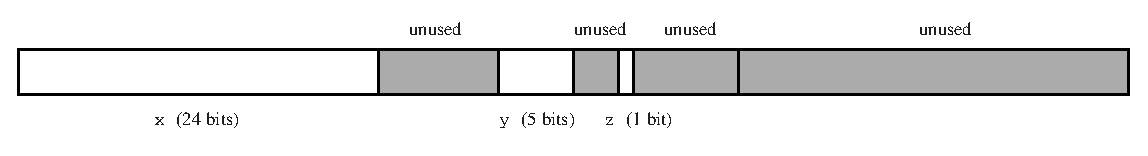
\includegraphics[scale=0.7]{Figures/standardAlignment.eps}\\
% ``Byte'' alignment byte-aligns the object and all fields:
% \hfill\raisebox{-1ex}[0pt][0pt]{\parbox[t]{3in}{
% \begin{samplecode}
% class A \{\\
% \>int x;  /* actual width 24 bits */\\
% \>byte y; /* actual width 5 bits */\\
% \>boolean z; /* actual width 1 bit */\\
% \}\\
% \end{samplecode}
% }}\\
% 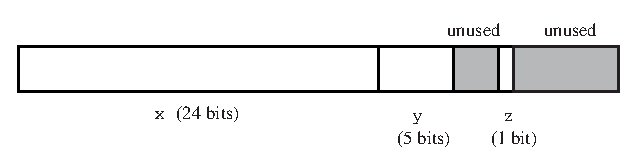
\includegraphics[scale=0.7]{Figures/byteAlignment.eps}\\
% ``Bit'' alignment requires no alignment of objects or fields:\\
% 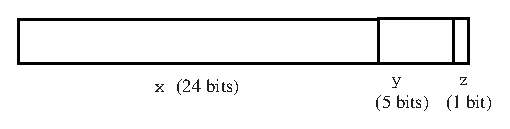
\includegraphics[scale=0.7]{Figures/bitAlignment.eps}\\
% \hline
% \end{tabular}

% Object header omitted.
% \end{slide}

%---------------------------------------------------------------------- SLIDE -
\begin{slide}{Field packing}
% converted with pngtopnm Figures/alignment.png | pnmtops -equalpixels -noturn > Figures/alignment.eps
\begin{center}
\vspace{0.75cm}
%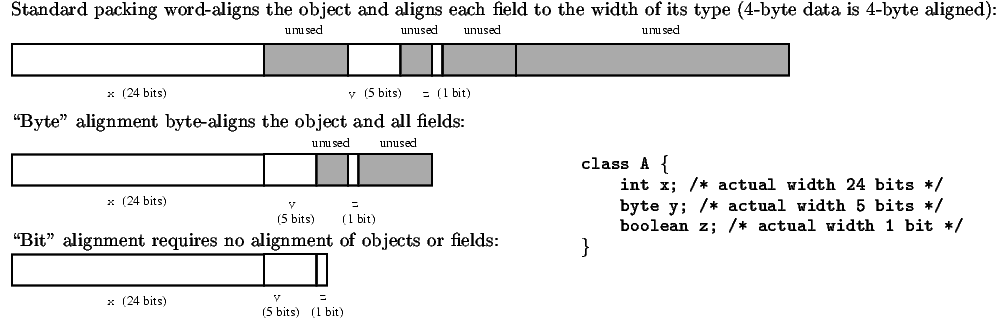
\includegraphics[scale=1.3]{Figures/alignment.eps}
\includegraphics[scale=0.35]{Figures/alignment2.eps}

\small Object header omitted.
\end{center}
\end{slide}

%---------------------------------------------------------------------- SLIDE -
\begin{slide}{How to compress objects} % just the second one

Three broad techniques:

\parbox[b]{2.5in}{%
\begin{itemize}%
\lightgray\renewcommand{\green}{\lightgray}% new bullet color
\item Field compression
\fieldelim\renewcommand{\green}{\fieldelim}% new bullet color
\item Mostly-constant field elimination
\lightgray\renewcommand{\green}{\lightgray}% new bullet color
\item Header optimizations
\renewcommand{\green}{\yellow} % restore yellow bullet color
\end{itemize}
}%
\parbox[b]{1.75in}{%
\hspace*{0.106in}\includegraphics[scale=0.4]{oqedraw/how-fieldelim-bbox.eps}%
}%
\end{slide}

%---------------------------------------------------------------------- SLIDE -
\overlays{6}{
\begin{slide}{Mostly-constant field elimination}
\begin{itemize}
 \item It's easy to remove {\yellow constant} fields.
 \fromSlide{2}{
 \item Key idea: remove {\yellow mostly} constant fields.
 \fromSlide{3}{
 \begin{itemize}
  \item \bp{\yellow Identify} fields which have a certain value ``most of
        the time''.
  \fromSlide{4}{
  \begin{itemize}
   \item Static analysis/Profiling
  \end{itemize}
  \fromSlide{5}{
  \item \bp{\yellow Transform} objects to remove fields w/ the common
        value.
  \fromSlide{6}{
  \begin{itemize}
   \item Static specialization/externalization.
  \end{itemize}
  }}}
 \end{itemize}
 }}
\end{itemize}
\end{slide}
}

%---------------------------------------------------------------------- SLIDE -
\begin{slide}{Static specialization}
\begin{itemize}
\item Split class implementations into ``field-less'' and
  ``field-ful'' versions.
\item Use virtual accessor functions to hide this split from users of
  the class.
\item Done at compile time, on fields which can be shown to be
  compile-time constants, thus ``static''.
\item Profiling guides splitting order if there are multiple candidate fields.
\end{itemize}
\end{slide}

%---------------------------------------------------------------------- SLIDE -
\overlays{2}{
\begin{slide}{Specialization example:\\\small java.lang.String}
\fontsize{9}{9}%
\newcommand{\myOffset}{\onlySlide*{1}{\makebox[0pt][l]{offset}}\onlySlide{2}{{\yellow getOffset()}}}%
\begin{samplecode}%
public final class String \{\\
\>private final char value[];\\
\onlySlide*{2}{\pnode{offl}}%
\>private final int offset;\onlySlide*{2}{\pnode{offr}}\\
\>private final int count;\\
\onlySlide{2}{\>\yellow protected int getOffset() \{ return 0; \}}\\
\>\ldots\\
\>public char charAt(int i) \{\\
\>\>return value[\myOffset{}+1];\\
\>\}\\
\>public String substring(int start) \{\\
\>\>int noff = \myOffset{} + start;\\
\>\>int ncnt = count - start;\\
\>\>return new String(value, noff, ncnt);\\
\>\}\\
\}\\
\end{samplecode}
\onlySlide*{2}{\ncline[linecolor=red,linewidth=2pt]{offl}{offr}}%
\end{slide}
}

%---------------------------------------------------------------------- SLIDE -
\begin{slide}{Specialization example:\\\small java.lang.String}
\fontsize{9}{9}%
\begin{samplecode}%
public final class {\yellow SmallString} \{\\
\>private final char value[];\\
\>\\  
\>private final int count;\\
\>protected int getOffset() \{ return 0; \}\\
\>\ldots\\
\>public char charAt(int i) \{\\
\>\>return value[getOffset()+i];\\
\>\}\\
\>\ldots\\
\}\\
public final class {\yellow String extends SmallString} \{\\
\>private final int {\yellow offset};\\
\>protected int {\yellow getOffset()} \{ return offset; \}\\
\}\\
\end{samplecode}
\end{slide}

%---------------------------------------------------------------------- SLIDE -
\newcommand{\myString}{\onlySlide*{1}{\makebox[0pt][l]{String}}\onlySlide{2}{{\yellow SmallString}}}%
\overlays{2}{
\begin{slide}{Transforming allocation sites}
Case 1: field is constant in constructor.

\fontsize{10}{10}%
\begin{samplecode}
String s = new \myString(new char[] \{'a', 'b', 'c'\});\\
\\
\myString(char[] val) \{\\
\>this.value = (char[]) val.clone();\\
\onlySlide*{2}{\pnode{offl2}}%
\>this.offset = 0;%
\onlySlide*{2}{\pnode{offr2}}\\
\>this.count = val.length;\\
\}\\
\end{samplecode}
\onlySlide*{2}{\ncline[linecolor=red,linewidth=2pt]{offl2}{offr2}}%
\end{slide}
}

%---------------------------------------------------------------------- SLIDE -
\overlays{2}{
\begin{slide}{Transforming allocation sites}
Case 2: field is simple function of constructor parameter.

\fontsize{10}{10}%
\begin{samplecode}%
\onlySlide*{1}{%
String s = new String(new char[] \{'a', 'b', 'c'\},\\
~~~~~~~~~~~~~~~~~~~~~~x, 1);\\
\\
String(char[] val, int offset, int length) \{\\
\>this.value = (char[]) val.clone();\\
\>this.offset = offset;\\
\>this.count = length;\\
\}\\
}%
\onlySlide*{2}{%
String s;\\
\\
if (x==0)\\
\>s = new {\yellow SmallString}(new char[] \{'a', 'b', 'c'\}, x, 1);\\
else\\
\>s = new {\yellow String}(new char[] \{'a', 'b', 'c'\}, x, 1);\\
}%
\end{samplecode}
\end{slide}
}

%---------------------------------------------------------------------- SLIDE -
\begin{slide}{Creating external fields}
\vspace{1cm}
\begin{itemize}
 \item Sometimes fields are {\yellow run-time} constants (or nearly so)
      but not {\yellow compile-time} constants.
 \begin{itemize}
  \item Examples: sparse matrices, ``two-input nodes'' in Jess expert
        system, the ``next'' field in short linked lists.
 \end{itemize}
 \item \bp{\yellow Exploit field$\rightarrow$map duality} to reduce memory
       overhead in the common case.
\end{itemize}
\end{slide}

%---------------------------------------------------------------------- SLIDE -
\overlays{3}{
\begin{slide}{Fields and Maps}
\begin{itemstep}
\item Accessing an object field {\tt a.b} (where {\tt a} is the object
  reference and {\tt b} is the field name) is equivalent to evaluating
  a map from \tuple{a, b} to the value type.
\item The mapping we will implement will be {\yellow incomplete}.  We
  define the result of accessing a non-existing mapping to be $\bot$.
\item To achieve our storage savings, we map $\bot$ to the frequent
  ``mostly-constant'' value.
\end{itemstep}
\end{slide}
}

%---------------------------------------------------------------------- SLIDE -
\begin{slide}{External map implementation}
\end{slide}

%---------------------------------------------------------------------- SLIDE -
\begin{slide}{We can do better!}
\end{slide}

%---------------------------------------------------------------------- SLIDE -
\overlays{3}{
\begin{slide}{Other details}
\begin{itemstep}
\item Use value profiling to identify classes where field
  externalization will be worthwhile.
\item In our experiments, looked for integer ``mostly-constant''
  values in the range $[-5,5]$ for numeric types.  Only looked at {\tt
    null} as a candidate for pointer types.
\item 0 and 1 by far the most common.
\end{itemstep}
\end{slide}
}

%---------------------------------------------------------------------- SLIDE -
\begin{slide}{How to compress objects} % just the third one

Three broad techniques:

\parbox[b]{2.5in}{%
\begin{itemize}%
\lightgray\renewcommand{\green}{\lightgray}% new bullet color
\item Field compression
\lightgray\renewcommand{\green}{\lightgray}% new bullet color
\item Mostly-constant field elimination
\headeropt\renewcommand{\green}{\headeropt}% new bullet color
\item Header optimizations
\renewcommand{\green}{\yellow} % restore yellow bullet color
\end{itemize}
}%
\parbox[b]{1.75in}{%
\includegraphics[scale=0.4]{oqedraw/how-header-bbox.eps}%
}%
\end{slide}

%---------------------------------------------------------------------- SLIDE -
\begin{slide}{Header optimizations:\\\small Hashcode/Lock compression}
\begin{center}
\vspace{.5cm}
\includegraphics[scale=0.6]{oqedraw/hashcomp-bbox.eps}
\end{center}
\end{slide}

%---------------------------------------------------------------------- SLIDE -
\begin{slide}{Header optimizations:\\\small Hashcode/Lock compression}
\end{slide}

%---------------------------------------------------------------------- SLIDE -
\begin{slide}{Header optimizations:\\\small claz compression}
\end{slide}

%---------------------------------------------------------------------- SLIDE -
\begin{slide}{Header optimizations:\\\small claz compression}
\end{slide}

%---------------------------------------------------------------------- SLIDE -
\begin{slide}{Class statistics}
\end{slide}

%---------------------------------------------------------------------- SLIDE -
\begin{slide}{How well does it work?}
\end{slide}

%---------------------------------------------------------------------- SLIDE -
\begin{slide}{Limitations \\ \small (read, ``future work'')}
\end{slide}

%---------------------------------------------------------------------- SLIDE -
\begin{slide}{Conclusions}
\end{slide}

%---------------------------------------------------------------------- SLIDE -
\part{The Graveyard Of Unused Slides follows this point.}

%---------------------------------------------------------------------- SLIDE -
\begin{slide}{Opportunities}
\end{slide}

%---------------------------------------------------------------------- SLIDE -
%\begin{slide}{Title here}
%\end{slide}

\end{document}

%%% Local Variables: 
%%% mode: latex
%%% TeX-master: t
%%% End: 
